% =========================================================================== %
% Yes. This is a document.

\documentclass[
	english,
	aspectratio=169,
	table
]{beamer}

% =========================================================================== %
% Theme
\usepackage{scrlfile}
	\ReplacePackage{beamerthemeSHUR}{./sty/beamerthemeSHUR}
	\ReplacePackage{beamerinnerthemefancy}{./sty/beamerinnerthemefancy}
	\ReplacePackage{beamerouterthemedecolines}{./sty/beamerouterthemedecolines}
	\ReplacePackage{beamercolorthemechameleon}{./sty/beamercolorthemechameleon}

\usetheme[
	pageofpages=von,
	bullet=circle,
	titleline=true,
	alternativetitlepage=true,
	watermark="",
	watermarkheight=0px,
	watermarkheightmult=0
	]
{SHUR}

% =========================================================================== %
% the usual stuff

\usepackage[utf8]{inputenc}
\usepackage[T1]{fontenc}
\usepackage{babel}
\usepackage{lmodern}
\usepackage{microtype}
\usepackage{csquotes}

\usepackage{tabularx}
\usepackage{booktabs}
\usepackage{multirow}

\usepackage{color, colortbl}
\usepackage{xcolor}
	\definecolor{tabhighlight}{RGB}{230,240,255}
	\definecolor{tabcontrast} {RGB}{200,210,255}

\usepackage{tabto}
\usepackage{xspace}

% math
\usepackage{amsmath}
\usepackage{amssymb}
\usepackage{dsfont}
\usepackage[arrowdel]{physics}
\usepackage{mathtools}

\usepackage{minted}
	\usemintedstyle{friendly}

\usepackage{tikz}
	\usetikzlibrary{positioning}
	\usetikzlibrary{matrix}
	\usetikzlibrary{shapes.geometric}
	\usetikzlibrary{backgrounds}
	\usetikzlibrary{calc}
	\usetikzlibrary{decorations.pathreplacing}
	\usetikzlibrary{arrows}
\usepackage{adjustbox}

\usepackage[most]{tcolorbox}
	\tcbsetforeverylayer
		{colback=cyan!10!white,
		 colframe=cyan!75!black,
		 arc=0pt,
		 outer arc=0pt
		}
	\newtcolorbox{codebox}[1][Code]
		{colback=black!5!white,
		 colframe=blue!40!black,
		 title=#1,
		 leftupper=6mm
		}
	\newtcolorbox{cmdbox}[1][Kommandozeilen-Befehl]
		{colback=black,
		 coltext=white,
		 fontupper=\ttfamily ,
		 colframe=blue!40!black,
		 title=#1,
		 outer arc=0pt
		}
	\newtcolorbox{warnbox}[1][Beachte]
		{colback=black!5!white,
		 colframe=red!40!black,
		 title=#1
		}
	\newtcolorbox{hintbox}[1][Tipp]
		{colback=black!5!white,
		 colframe=green!40!black,
		 title=#1
		}
	\newenvironment{itembox}
		{\begin{tcolorbox}\begin{itemize}}%
		{\end{itemize}\end{tcolorbox}}
	\newtcolorbox{doublebox}[1][.3]
		{righthand width=#1\linewidth,
		 sidebyside,
		 sidebyside gap=6mm,
		 sidebyside align=center,
		 lower separated=false}
	
%==============================================================================%
% GLOBAL MACROS

\newcommand*{\eg}{e.\,g. }
\newcommand*{\ie}{i.\,e. }

\newcommand{\Thus}{\ensuremath{\Rightarrow}\xspace}
\newcommand{\thus}{\ensuremath{\rightarrow}\xspace}

\newcommand*{\tabcrlf}{\\ \midrule}			% actually still allows for optional argument

\newcommand*{\inPy}[1]{\mintinline{python3}{#1}}

% =========================================================================== %

\author{Stefan Hartinger}
\title{Programming in Python}
\subtitle{Part 10: Reading and Writing Files}
\institute{University Regensburg, Department of Theoretical Physics}
\date{Block Course, Summer Term 2021}

% =========================================================================== %

\begin{document}
% =========================================================================== %

\begin{frame}[t,plain]
\titlepage
\end{frame}

% =========================================================================== %

\begin{frame}[fragile]{Goal: Better Understand Python's Memory Management}
%
\begin{itemize}
\item Object Descriptor and Memory Models
\item Passing Variables to Functions
\item Recap: Mutable and Immutable Objects
\item \inPy{global} and \inPy{nonlocal}
\end{itemize}
%
\end{frame}

% =========================================================================== %

\begin{frame}[fragile]{Object Descriptor and Memory Models}
%
\begin{itemize}
\item Recap: For a computer, everything is numbers
\item Context needed for interpretation
\item Python needs to store that context \emph{somewhere}
\item Uniform format for stupid computers
\item \emph{Object Descriptor}
	\begin{itemize}
	\item Data Type ID (number that can be looked up in a table)
	\item Adress of actual data
	\item Size of actual data
	\item (More internal stuff...)
	\end{itemize}
\end{itemize}
%
\begin{hintbox}
Even what we think of as \emph{one} number is, internally, a whole bunch of numbers.
\end{hintbox}
%
\end{frame}

% =========================================================================== %\\

\begin{frame}[fragile]
%
\begin{tcolorbox}[title=Memory Model: \texttt{int}s]
What does \inPy{x = 1337} look like internally?
\vspace{20pt}
\begin{center}
\begin{tikzpicture}
  [ 
    cell/.style={text width=8mm,
      text height=4mm, draw=black, inner sep=1mm},
    ld/.style={draw=blue,shorten >=2pt,->}
  ]
  
  \node  (invisible) at (-2, -0.25) {};
  \node  (a0) at ( 0,0) [cell] {\ttfamily  ...};
  \node  (a1) at ( 1,0) [cell] {\ttfamily @int};
  \node  (a2) at ( 2,0) [cell] {\ttfamily @dat};
  \node  (a3) at ( 3,0) [cell] {\ttfamily  8  };
  \node  (a4) at ( 4,0) [cell] {\ttfamily  ...};
  \node  (a5) at ( 5,0) [cell] {\ttfamily  ...};
  \node  (a6) at ( 6,0) [cell] {\ttfamily 1337};
  \node  (a7) at ( 7,0) [cell] {\ttfamily  ...};
  
  \node (b0) [above=1mm of a0] {\tiny 0xEFF8};
  \node (b1) [above=1mm of a1, color=teal] {\tiny 0xF000};
  \node (b2) [above=1mm of a2] {\tiny 0xF008};
  \node (b3) [above=1mm of a3] {\tiny 0xF010};
  \node (b4) [above=1mm of a4] {\tiny 0xF018};
  \node (b5) [above=1mm of a5] {\tiny 0xF020};
  \node (b6) [above=1mm of a6] {\tiny 0xF028};
  \node (b7) [above=1mm of a7] {\tiny 0xF030};
  
  \draw [decorate, decoration={brace,amplitude=7pt}, xshift=-0pt, yshift=0pt]
  		(+0.5, 1.0) -- ( 4.5, 1.0) node (x) [midway, yshift=+0.5cm] 
		(braceDescriptor) {Descriptor of \texttt{x}};
	
  \draw [decorate, decoration={brace,amplitude=7pt}, xshift=-0pt, yshift=0pt]
  		( 5.5, 1.0) -- ( 6.5, 1.0) node (y) [midway, yshift=+0.5cm] 
		(braceContent) {Use data of \texttt{x}};

	\draw [->, bend right=20]
		(a2.south) to node 
		[below] {cell content: 0xF028} 
		(a6.south);
			
	\draw [->, bend left=20]
		(a1.south) to node 
		[below] {cell content: ID of class \inPy{int}} 
		(invisible.south);
		
\end{tikzpicture}
\end{center}

\vspace{20pt}
Internally, \texttt{x} is only the \emph{address of the descriptor}, \ie the value \texttt{0xF000}.\\
Any access to the \emph{value of \texttt{x}} goes through a series of interpreteation steps!
\end{tcolorbox}
%
\end{frame}

% =========================================================================== %\\

\begin{frame}[fragile]
%
\begin{tcolorbox}[title=Memory Model: \texttt{list}s]
What does \inPy{lst = [x, 666]} look like internally?
\vspace{10pt}
\begin{center}
\begin{tikzpicture}
  [ 
    cell/.style={text width=8mm,
      text height=4mm, draw=black, inner sep=1mm},
    ld/.style={draw=blue,shorten >=2pt,->}
  ]
  
  \node  (invisible) at (-2, -0.25) {};
  \node  (a0) at ( 0,0) [cell] {\ttfamily  ...};
  \node  (a1) at ( 1,0) [cell] {\ttfamily @lst};
  \node  (a2) at ( 2,0) [cell] {\ttfamily @dat};
  \node  (a3) at ( 3,0) [cell] {\ttfamily  16 };
  \node  (a4) at ( 4,0) [cell] {\ttfamily  ...};
  \node  (a5) at ( 5,0) [cell] {\ttfamily  ...};
  \node  (a6) at ( 6,0) [cell] {\ttfamily @x  };
  \node  (a7) at ( 7,0) [cell] {\ttfamily @new};
  \node  (a8) at ( 8,0) [cell] {\ttfamily  ...};
  
  \node (b0) [above=1mm of a0] {\tiny 0xF030};
  \node (b1) [above=1mm of a1, color=teal] {\tiny 0xF000};
  \node (b2) [above=1mm of a2] {\tiny 0xF038};
  \node (b3) [above=1mm of a3] {\tiny 0xF040};
  \node (b4) [above=1mm of a4] {\tiny 0xF048};
  \node (b5) [above=1mm of a5] {\tiny 0xF050};
  \node (b6) [above=1mm of a6] {\tiny 0xF058};
  \node (b7) [above=1mm of a7] {\tiny 0xF060};
  \node (b8) [above=1mm of a8] {\tiny 0xF068};
  
  \draw [decorate, decoration={brace,amplitude=7pt}, xshift=-0pt, yshift=0pt]
  		(+0.5, 1.0) -- ( 4.5, 1.0) node (x) [midway, yshift=+0.5cm] 
		(braceDescriptor) {Descriptor of \texttt{lst}};
	
  \draw [decorate, decoration={brace,amplitude=7pt}, xshift=-0pt, yshift=0pt]
  		( 5.5, 1.0) -- ( 7.5, 1.0) node (y) [midway, yshift=+0.5cm] 
		(braceContent) {Use data of \texttt{lst}};

	\draw [->, bend right=20]
		(a2.south) to node 
		[below] {cell content: 0xF058} 
		(a6.south);
			
	\draw [->, bend left=20]
		(a1.south) to node 
		[below] {cell content: ID of class \inPy{list}}
		(invisible.south);
	
	\node (t6) at (6.8,-1.5) {\texttt{0xF028}};
	\node (t7) at (8.5,-1.5) {\texttt{0xF430}};
	
	\draw [->, bend right=15] (a6.south) to node [below] {} (t6.north);
	\draw [->, bend right=15] (a7.south) to node [below] {} (t7.north);
\end{tikzpicture}
\end{center}

\vspace{10pt}
The content of lists is actually only a series of adresses: each adress references an object descriptor, even for literal constants! For constants, like \inPy{666} a new object descriptor is constructed \emph{somewhere}. They have no (exposed) symbol.
\end{tcolorbox}
%
\end{frame}

% =========================================================================== %

\begin{frame}{Changing Values: Mutable and Immutable Objects}
%
\begin{itemize}
\item Recall: Most objects (so far): \emph{immutable}
\item Everything except for \inPy{list}s, \inPy{dict}s and \inPy{set}s
\item Effect of changing a variable depends on mutability
\item Immutables: Set up new descriptor, forget about old one
\item Mutables: Only change the content memory cell
\end{itemize}
%
\end{frame}

% =========================================================================== %

\begin{frame}[fragile]{Sublists and Changing References}
%
\begin{codebox}[Example: Changing Values]
\begin{minted}[linenos, fontsize=\scriptsize]{python3}
a, b, c = 1, 2, 3
lst = [[a, b], c]

c = 5

print(lst)
print(c)
\end{minted}
\end{codebox}
%
\begin{cmdbox}[Output: Changing Values]
\begin{minted}[fontsize=\scriptsize]{text}
[[1, 2], 3]
5
\end{minted}
\end{cmdbox}
%
\end{frame}

% =========================================================================== %

\begin{frame}[fragile]{Analyzing Memory: Sublists and Changing References}
%
\mint{python3}{a, b, c = 1, 2, 3}
\mint{python3}{list = [[a, b], c]}
%
\begin{tcolorbox}[title=Memory Model]
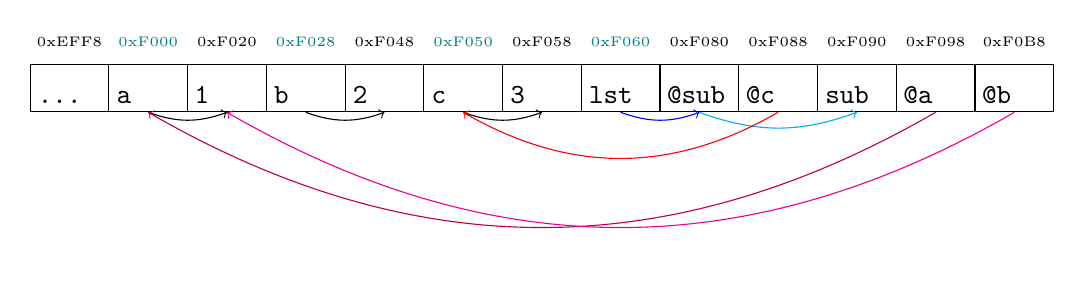
\begin{tikzpicture}
  [ 
    cell/.style={text width=8mm,
      text height=4mm, draw=black, inner sep=1mm},
    ld/.style={draw=blue,shorten >=2pt,->}
  ]
  
  \node  (a0)  at ( 0,0) [cell] {\ttfamily  ...};
  \node  (a1)  at ( 1,0) [cell] {\ttfamily a   };
  \node  (a2)  at ( 2,0) [cell] {\ttfamily 1   };
  \node  (a3)  at ( 3,0) [cell] {\ttfamily b   };
  \node  (a4)  at ( 4,0) [cell] {\ttfamily 2   };
  \node  (a5)  at ( 5,0) [cell] {\ttfamily c   };
  \node  (a6)  at ( 6,0) [cell] {\ttfamily 3   };
  \node  (a7)  at ( 7,0) [cell] {\ttfamily lst };
  \node  (a8)  at ( 8,0) [cell] {\ttfamily @sub};
  \node  (a9)  at ( 9,0) [cell] {\ttfamily @c  };
  \node  (a10) at (10,0) [cell] {\ttfamily sub };
  \node  (a11) at (11,0) [cell] {\ttfamily @a  };
  \node  (a12) at (12,0) [cell] {\ttfamily @b  };
  
  \node (b0)  [above=1mm of a0]  {\tiny 0xEFF8};
  \node (b1)  [above=1mm of a1, color=teal] {\tiny 0xF000};
  \node (b2)  [above=1mm of a2]  {\tiny 0xF020};
  \node (b3)  [above=1mm of a3, color=teal]  {\tiny 0xF028};
  \node (b4)  [above=1mm of a4] {\tiny 0xF048};
  \node (b5)  [above=1mm of a5, color=teal]  {\tiny 0xF050};
  \node (b6)  [above=1mm of a6]  {\tiny 0xF058};
  \node (b7)  [above=1mm of a7, color=teal]  {\tiny 0xF060};
  \node (b8)  [above=1mm of a8]  {\tiny 0xF080};
  \node (b9)  [above=1mm of a9]  {\tiny 0xF088};
  \node (b10) [above=1mm of a10] {\tiny 0xF090};
  \node (b11) [above=1mm of a11] {\tiny 0xF098};
  \node (b12) [above=1mm of a12] {\tiny 0xF0B8};
  
  
	\draw [->, bend right=20]
		(a1.south) to node 
		[below] {} 
		(a2.south);
		
	\draw [->, bend right=20]
		(a3.south) to node 
		[below] {} 
		(a4.south);
		
	\draw [->, bend right=20]
		(a5.south) to node 
		[below] {} 
		(a6.south);
		
	\draw [->, bend right=20, color=blue]
		(a7.south) to node 
		[below] {} 
		(a8.south);
		
		
	\draw [->, bend right=20, color=cyan]
		(a8.south) to node 
		[below] {} 
		(a10.south);
		
		
	\draw [->, bend left=30, color=red]
		(a9.south) to node 
		[below] {} 
		(a5.south);
		
		
	\draw [->, bend left=30, color=purple]
		(a11.south) to node 
		[below] {} 
		(a1.south);
		
	\draw [->, bend left=30, color=magenta]
		(a12.south) to node 
		[below] {} 
		(a2.south);
\end{tikzpicture}
\end{tcolorbox}
%
\end{frame}

% =========================================================================== %

\begin{frame}{Changing References}
%
\begin{itemize}
\item \texttt{c} is \inPy{int} and thus \emph{immutable}
\item Line 4 (\texttt{c = 5}) requires \emph{new construction of an \inPy{int}!}
\item This does not affect the contents \texttt{lst}!
	\begin{itemize}
	\item \enquote{New} \texttt{c}, somewhere in memory
	\item Symbol \texttt{c} refers to new location
	\item Maintain \enquote{old} descriptor
	\item \texttt{lst} still references old descriptor
	\end{itemize}
\end{itemize}
%
\end{frame}

% =========================================================================== %

\begin{frame}{Recap: Calling Functions}
%
\begin{itemize}
\item Functions have their own \enquote{working environment}
\item Own list of symbols (like \texttt{x}) pointing to descriptors \emph{somewhere}
\item Function arguments: part of this \emph{local} list
\item Initialized with a reference
\end{itemize}
%
\end{frame}

% =========================================================================== %

\begin{frame}[fragile]
%
\begin{tcbraster}[raster columns=3,
                  raster equal height,
                  nobeforeafter,
                  raster column skip=0.5cm]
\begin{codebox}[A Function Call]
\begin{minted}[linenos, fontsize=\scriptsize]{python3}
def func(a) :
    b = 2
    c = 3
    print(x, a, b, c)

x = 1
func(x)
\end{minted}
\end{codebox}
%
\begin{tcolorbox}[title=Symbol Table \texttt{main}]
\scriptsize
\begin{tabular}{cc}
	\textbf{Symbol} & \textbf{Adress} \tabcrlf
	\texttt{x} & \texttt{0xF000}
\end{tabular}
\end{tcolorbox}
%
\begin{tcolorbox}[title=Symbol Table \texttt{func}]
\scriptsize
\begin{tabular}{cc}
	\textbf{Symbol} & \textbf{Adress} \tabcrlf
	\texttt{x} & \texttt{0xF000} \\
	\texttt{a} & \texttt{0xF000} \\
	\texttt{b} & \texttt{0xF018} \\
	\texttt{c} & \texttt{0xF030} \\	
\end{tabular}
\end{tcolorbox}
\end{tcbraster}
%
\begin{tcolorbox}[title=Memory Model]
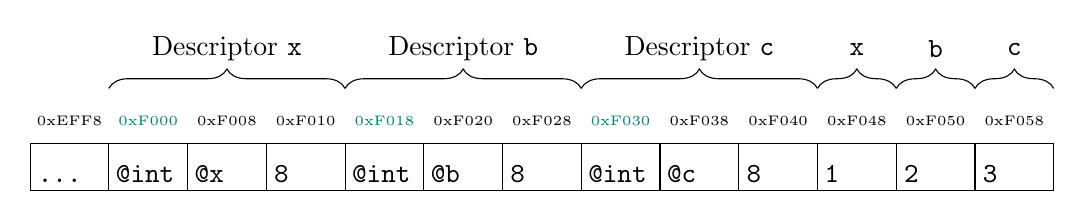
\begin{tikzpicture}
  [ 
    cell/.style={text width=8mm,
      text height=4mm, draw=black, inner sep=1mm},
    ld/.style={draw=blue,shorten >=2pt,->}
  ]
  
  \node  (a0)  at ( 0,0) [cell] {\ttfamily  ...};
  \node  (a1)  at ( 1,0) [cell] {\ttfamily @int};
  \node  (a2)  at ( 2,0) [cell] {\ttfamily @x  };
  \node  (a3)  at ( 3,0) [cell] {\ttfamily 8   };
  \node  (a4)  at ( 4,0) [cell] {\ttfamily @int};
  \node  (a5)  at ( 5,0) [cell] {\ttfamily @b  };
  \node  (a6)  at ( 6,0) [cell] {\ttfamily 8   };
  \node  (a7)  at ( 7,0) [cell] {\ttfamily @int};
  \node  (a8)  at ( 8,0) [cell] {\ttfamily @c  };
  \node  (a9)  at ( 9,0) [cell] {\ttfamily 8   };
  \node  (a10) at (10,0) [cell] {\ttfamily 1   };
  \node  (a11) at (11,0) [cell] {\ttfamily 2   };
  \node  (a12) at (12,0) [cell] {\ttfamily 3   };
  
  \node (b0)  [above=1mm of a0]  {\tiny 0xEFF8};
  \node (b1)  [above=1mm of a1, color=teal] {\tiny 0xF000};
  \node (b2)  [above=1mm of a2]  {\tiny 0xF008};
  \node (b3)  [above=1mm of a3]  {\tiny 0xF010};
  \node (b4)  [above=1mm of a4, color=teal] {\tiny 0xF018};
  \node (b5)  [above=1mm of a5]  {\tiny 0xF020};
  \node (b6)  [above=1mm of a6]  {\tiny 0xF028};
  \node (b7)  [above=1mm of a7, color=teal]  {\tiny 0xF030};
  \node (b8)  [above=1mm of a8]  {\tiny 0xF038};
  \node (b9)  [above=1mm of a9]  {\tiny 0xF040};
  \node (b10) [above=1mm of a10] {\tiny 0xF048};
  \node (b11) [above=1mm of a11] {\tiny 0xF050};
  \node (b12) [above=1mm of a12] {\tiny 0xF058};
  
  \draw [decorate, decoration={brace,amplitude=7pt}, xshift=-0pt, yshift=0pt]
  		(+0.5, 1.0) -- ( 3.5, 1.0) node (x) [midway, yshift=+0.5cm] 
		(braceDescriptor) {Descriptor \texttt{x}};
  \draw [decorate, decoration={brace,amplitude=7pt}, xshift=-0pt, yshift=0pt]
  		(+3.5, 1.0) -- ( 6.5, 1.0) node (x) [midway, yshift=+0.5cm] 
		(braceDescriptor) {Descriptor \texttt{b}};
  \draw [decorate, decoration={brace,amplitude=7pt}, xshift=-0pt, yshift=0pt]
  		(+6.5, 1.0) -- ( 9.5, 1.0) node (x) [midway, yshift=+0.5cm] 
		(braceDescriptor) {Descriptor \texttt{c}};

  \draw [decorate, decoration={brace,amplitude=7pt}, xshift=-0pt, yshift=0pt]
  		(+ 9.5, 1.0) -- (10.5, 1.0) node (x) [midway, yshift=+0.5cm] 
		(braceDescriptor) {\texttt{x}};
  \draw [decorate, decoration={brace,amplitude=7pt}, xshift=-0pt, yshift=0pt]
  		(+10.5, 1.0) -- (11.5, 1.0) node (x) [midway, yshift=+0.5cm] 
		(braceDescriptor) {\texttt{b}};
  \draw [decorate, decoration={brace,amplitude=7pt}, xshift=-0pt, yshift=0pt]
  		(+11.5, 1.0) -- (12.5, 1.0) node (x) [midway, yshift=+0.5cm] 
		(braceDescriptor) {\texttt{c}};
\end{tikzpicture}
\end{tcolorbox}
%
Symbol tables often go by the name of \emph{binding}.
%
\end{frame}

% =========================================================================== %

\begin{frame}{Nonlocal References}
%
\begin{itemize}
\item Previous example: \texttt{a}, \texttt{b}, \texttt{c} are not visible on module level
\item But: \texttt{x} is visible within \texttt{func}
\item \emph{Nonlocal} reference
\item Rule of thumb: Hiearchical structure gives resolution: variables in higher level scopes are more visible
\item Different \emph{binding} depending on access to the variable
	\begin{itemize}
	\item Only read access: try to bind symbol to a higher level object
	\item Example: \texttt{x} in previous code
	\item Write access: create a \emph{new local variable}.
	\end{itemize}
\end{itemize}
%
\end{frame}

% =========================================================================== %

\begin{frame}[fragile]
%
\begin{tcbraster}[raster columns=2,
                  raster equal height,
                  nobeforeafter,
                  raster column skip=0.5cm]
\begin{codebox}[Example: Nonlocal Variables (1)]
\begin{minted}[fontsize=\scriptsize, linenos]{python3}
def foo (param) :
    localVar = -1

    print("In foo:")
    print(param)
    print(moduleLevel)
    print(localVar)
    print()

moduleLevel = 1
localVar    = 1

foo(1)

print("In module level:")
print(moduleLevel)
print(localVar)
\end{minted}
\end{codebox}
%
\begin{cmdbox}[Output: Nonlocal Variables (1)]
\begin{minted}[fontsize=\scriptsize]{text}
In foo:
1
1
-1

In module level:
1
1
\end{minted}
\end{cmdbox}
\end{tcbraster}
%
\Thus~Two different bindings for symbol \texttt{localVar}, depending on context\\
\phantom{.}\qquad(in \texttt{foo} or in module level)
%
\end{frame}

% =========================================================================== %

\begin{frame}[fragile]
%
\begin{tcbraster}[raster columns=2,
                  raster equal height,
                  nobeforeafter,
                  raster column skip=0.5cm]
\begin{warnbox}[Example: Nonlocal Variables (2), leftupper=7mm]
\begin{minted}[fontsize=\scriptsize, linenos]{python3}
def foo () :
    print(moduleLevel)
    
    moduleLevel = -1

moduleLevel = 1

foo()

print(moduleLevel)

\end{minted}
\end{warnbox}
%
\begin{cmdbox}[Output: Nonlocal Variables (2)]
\begin{minted}[fontsize=\scriptsize]{text}
Traceback (most recent call last):

  File "/home/blue-chameleon/.config/
        spyder-py3/temp.py", line 8, 
        in <module>
    foo()

  File "/home/blue-chameleon/.config/
        spyder-py3/temp.py", line 2,
        in foo
    print(moduleLevel)

UnboundLocalError: local variable 
    'moduleLevel' referenced before
    assignment
\end{minted}
\end{cmdbox}
\end{tcbraster}
%
\begin{itemize}
\item Write access (line 4) makes \texttt{moduleLevel} a \emph{local} variable
\item Undefined at first read access (line 2)
\item[\Thus] Error message
\end{itemize}
%
\end{frame}

% =========================================================================== %

\begin{frame}[fragile]{\inPy{global} Declaration}
%
\begin{itemize}
\item To make the previous example work: Tell Python to bind \texttt{moduleLevel} to variable on module level
\item New command: \inPy{global moduleLevel}
\item Allows changes to module level
\item (Don't you ever use it)
\end{itemize}
%
\end{frame}

% =========================================================================== %

\begin{frame}[fragile]
%
\begin{tcbraster}[raster columns=2,
                  raster equal height,
                  nobeforeafter,
                  raster column skip=0.5cm]
\begin{codebox}[Example: Nonlocal Variables (3)]
\begin{minted}[fontsize=\scriptsize, linenos]{python3}
def foo () :
    global moduleLevel
    print("in foo, before change",
          moduleLevel)
    
    moduleLevel = -1

moduleLevel = 1

foo()

print("in module level, after change",
      moduleLevel)
\end{minted}
\end{codebox}
%
\begin{cmdbox}[Output: Nonlocal Variables (3)]
\begin{minted}[fontsize=\scriptsize]{text}
in foo, before change 1
in module level, after change -1
\end{minted}
\end{cmdbox}
\end{tcbraster}
%
\begin{itemize}
\item \inPy{global} declaration (line 2) binds both symbols ($\texttt{moduleLevel}_{\text{foo}}$ and $\texttt{moduleLevel}_{\text{main}}$) to the same descriptor
\item Read- and write-access as if on module level!
\end{itemize}
%
\end{frame}

% =========================================================================== %

\begin{frame}[fragile]{\inPy{nonlocal} Declaration}
%
\begin{itemize}
\item Essentially the same for nested functions
\item Make binding to one level higher, but not module level
\item Surprisingly more useful than \inPy{global}
\item (You likely won't need it very often, though)
\end{itemize}
%
\end{frame}

% =========================================================================== %

\begin{frame}[fragile]
%
\begin{codebox}[Example: \texttt{nonlocal}]
\begin{minted}[linenos, fontsize=\scriptsize]{python3}
def doesSomethingComplicated () :
    result = ""
    def someSubProblem () :
        nonlocal result
        initialState = len(result)
        result += "A partially solved problem starting at " + str(initialState)
    
    someSubProblem()
    print(result)
    result = result.replace("partially", "completely")
    return result

print( doesSomethingComplicated() )
\end{minted}
\end{codebox}
%
\begin{cmdbox}[Output: \texttt{nonlocal}]
\begin{minted}[fontsize=\scriptsize]{text}
A partially solved problem starting at 0
A completely solved problem starting at 0
\end{minted}
\end{cmdbox}
%
\end{frame}

% =========================================================================== %

\begin{frame}{Best Practice}
%
\begin{itemize}
\item Forget about \inPy{global} and \inPy{nonlocal}
\item Only input to functions: parameter list
\item Only output from functions: \inPy{return} statement
\item Updating a variable by a function: \inPy{variable = function(variable)}
\item (Possible) exception: mutable variables like lists
\item \inPy{updateFunction(myList)}
\item Make sure the function name reflects this behaviour
	\begin{itemize}
	\item Good names: \texttt{updateXXX}, \texttt{appendThings}, \texttt{removeThings}, \texttt{clear}, ...
	\item Okay, possibly ambiguous name: \texttt{filter} (updating behaviour not implicitly clear)
	\item[\Thus] Function Names should be verbs!
	\end{itemize}
\end{itemize}
%
\end{frame}

% =========================================================================== %

\begin{frame}[fragile]
%
\begin{codebox}[Example: appendUniqueChars]
\begin{minted}[linenos, fontsize=\scriptsize]{python3}
def appendUniqueChars (queue, string) :
    for char in string :
        if not char in queue :
            queue.append(char)

data = []
appendUniqueChars(data, "The quick brown fox jumps over the lazy dog")
appendUniqueChars(data, "This will add only an exclamation mark!")
print(data)
\end{minted}
\end{codebox}
%
\begin{cmdbox}[Output: \texttt{nonlocal}]
\begin{minted}[fontsize=\scriptsize]{text}
['T', 'h', 'e', ' ', 'q', 'u', 'i', 'c', 'k', 'b', 'r', 'o', 'w', 'n', 'f', 'x',
 'j', 'm', 'p', 's', 'v', 't', 'l', 'a', 'z', 'y', 'd', 'g', '!']
\end{minted}
\end{cmdbox}
%
\begin{hintbox}
You should do this with \inPy{set}s, ideally.
\end{hintbox}
%
\end{frame}
\end{document}

% MAREI!!
% whom do I give credit? Where?